\subsubsection{Giới thiệu bộ dữ liệu}
    \paragraph{Nguồn dữ liệu}
    \leavevmode

    Bộ dữ liệu được thu thập bằng Jikan api, nguồn cơ sở dữ liệu website myanimelist.net 

    \paragraph{Mô tả dữ liệu}
    \leavevmode

    Đây là bộ dữ liệu chức thông tin các bộ phim và sản phẩm phương tiện truyền thông liên quan đến hoạt hình Nhật Bản, được cập nhật cho đến tháng 6 năm 2025 từ cơ sở dữ liệu của website My Anime List (MAL). Mỗi dòng dữ liệu chứa thông tin về bộ phim kèo theo thông tin đánh giá, nhận xét của người dùng.

    Ví dụ một phần dữ liệu:

    \begin{CJK}{UTF8}{gbsn}
    \begin{table}[htbp]
    \centering
    \caption{Một phần bảng dữ liệu MAL dataset}
    \label{tab:stat-mal-exp}
        \begin{tabular}{|r|p{3cm}|p{2.75cm}|r|p{1.6cm}|r|r|r|r|}
        \hline
        mal\_id & title\_english & title\_japanese & type & status & score & rank & members & ... \\
        \hline
        33352 & Violet Evergarden & ヴァイオレット・エヴァーガーデン & TV & Finished Airing & 8.68 & 67 & 1,904,842 & ... \\
        \hline
        35677 & Liz and the Blue Bird & リズと青い鳥 & Movie & Finished Airing & 8.22 & 375 & 154,915 & ... \\
        \hline
        41457 & 86 Eighty-Six & 86―エイティシックス― & TV & Finished Airing & 8.33 & 255 & 890,163 & ... \\
        \hline
        52991 & Frieren: Beyond Journey's End & 葬送のフリーレン & TV & Finished Airing & 9.3 & 1 & 1,140,504 & ... \\
        \hline
        ... & ... & ... & ... & ... & ... & ... & ... & ... \\
        \hline
        \end{tabular}

    \end{table}
    \end{CJK}

    \FloatBarrier

     Bộ dữ liệu có 28,707 dòng, bao gồm 20 cột như sau:
     \begin{itemize}
        \item Kiểu dữ liệu: \textbf{Qualitative} 

        \begin{enumerate}
            \item \textbf{title}: Tên (chung, có thể là dịch hoặc phiên âm)
            \item \textbf{title\_english}: Tên dịch tiếng Anh
            \item \textbf{title\_japanese}: Tên gốc tiếng Nhật
            \item \textbf{type}: Thể loại
            
                Có các giá trị: 
                \begin{itemize}
                    \item TV: Phim chiếu TV
                    \item Movie: Phim chiếu rạp
                    \item Special: Phần đặc biệt
                    \item OVA: Phần đặc biệt (tặng kèm DVD, Blu-ray...)
                    \item TV Special: Phần đặc biệt (chiếu TV)
                    \item ONA: Phát trực tuyến 
                    \item Music: Âm nhạc
                    \item CM: Quảng cáo (TV, ...)
                    \item PV: Quảng cáo (trailer, teaser...)
                \end{itemize}

            \item \textbf{status}: Tình trạng chiếu
            
                Có các giá trị: 
                \begin{itemize}
                    \item Finished Airing: Đã chiếu hết

                    \item Currently Airing: Đang chiếu

                    \item Not yet aired: Sắp chiếu
                \end{itemize}

            \item \textbf{synopsis}: Tóm tắt nội dung

            \item \hypertarget{line:mal-genres}{\textbf{genres}}: Thể loại, chuỗi danh sách ngăn cách bởi dấu ','

            \item \textbf{themes}: Chủ đề chính, chuỗi danh sách ngăn cách bởi dấu ','

            \item \textbf{demographics}: Đối tượng khán giả, chuỗi danh sách ngăn cách bởi dấu ','

            \item \textbf{studios}: Tên xưởng phim thực hiện

            \item \textbf{url}: Đường dẫn trang web của dòng hiện tại
            
        \end{enumerate}

        \item Kiểu dữ liệu: \textbf{Quantitative} 
        \begin{itemize}
            \item \textbf{Discrete}:

                \begin{enumerate}[resume]
                    \item \textbf{mal\_id}: ID phim trong cơ sở dữ liệu

                    \item  \textbf{episodes}: Số tập


                    \item \textbf{members}: Số người theo dõi (đang xem, đã xem)

                    \item \textbf{favorites}: Số người đánh giá yêu thích (Mỗi tài khoản chỉ có thể chọn yêu thích tối đa 10, 20 nếu là tài khoản trả phí)
                    
                    \item \textbf{rank}: Xếp hạng (theo đánh giá)
                    
                    \item \textbf{popularity}: Xếp hạng (theo số người theo dõi)

                    \item \textbf{year}: Năm bắt đầu chiếu

                \end{enumerate}

            \item \textbf{Continuous}:

                \begin{enumerate}[resume]
                    \item \textbf{score}: Điểm đánh giá trung bình tất cả đánh giá. Thang 0-10

                    \item \textbf{aired\_date}: Ngày bắt đầu chiếu
                \end{enumerate}
        \end{itemize}
     
     \end{itemize}

\subsubsection{Các nghiên cứu liên quan}
    Jesús Armenta-Segura và Grigori Sidorov \cite{armenta2023anime}, các phương pháp học máy truyền thống đã được ứng dụng nhằm dự đoán mức độ thành công của các bộ anime ngay từ giai đoạn phát triển ban đầu. Tác giả đã xây dựng AniSyn7 – một tập dữ liệu gồm 6.928 tóm tắt nội dung phim hoạt hình, được gán nhãn nhị phân (thành công/không thành công) dựa trên điểm số từ MyAnimeList. Nghiên cứu đã triển khai ba bộ phân loại học máy phổ biến gồm Máy vector hỗ trợ (SVM), Naive Bayes và Hồi quy Logistic, kết hợp với các phương pháp vector hóa như Bag of Words, n-grams và cây phụ thuộc cú pháp. Kết quả cho thấy, mô hình BBTC (kết hợp BoW, bigram, trigram và trigram ký tự) sử dụng SVM hoặc Logistic Regression đạt F1-score cao nhất là 0.55. Điều này chứng minh rằng các đặc trưng ngôn ngữ trong phần tóm tắt nội dung có thể mang lại giá trị đáng kể trong việc dự đoán thành công của anime. Nghiên cứu không chỉ cung cấp một tập dữ liệu nền tảng cho các nghiên cứu sau này mà còn mở ra tiềm năng mở rộng theo hướng đa nhiệm hoặc đa phương thức, bao gồm cả phân tích hình ảnh và kỹ thuật học sâu hiện đại nhằm nâng cao độ chính xác và khả năng ứng dụng trong thực tiễn.

    Trong nghiên cứu của Nathanael Setiawan và cộng sự \cite{setiawan2023time}, mô hình chuỗi thời gian Prophet được áp dụng nhằm dự đoán xu hướng phổ biến của các thể loại anime trong tương lai. Dựa trên dữ liệu từ MyAnimeList, nhóm nghiên cứu sử dụng Prophet để phân tích sự thay đổi mức độ phổ biến theo thời gian, đạt RMSE 1.102 và MAPE 13.551\%. Kết quả cho thấy các thể loại như Super Power, Demons và Supernatural sẽ tiếp tục tăng trưởng đến năm 2025, trong khi Josei, Cars và Kids giảm mạnh. Nghiên cứu này là một trong số ít ứng dụng chuỗi thời gian trong lĩnh vực anime, hỗ trợ các nhà sản xuất và nhóm nội địa hóa định hướng phát triển thể loại phù hợp với thị hiếu toàn cầu.

\subsubsection{Phân tích dữ liệu}
    \paragraph{Tiền xử lý}
    \leavevmode

    Trước tiên, nhóm thực hiện một số bước tiền xử lý bộ dữ liệu thô như sau:

    \begin{itemize}
        \item  Bộ dữ liệu không chứa thông tin bình luận đánh giá. Nhóm sử dụng cùng api nguồn dữ liệu để thu thập thêm thông tin bình luận, đánh giá như sau:

        Thu thập dữ liệu tạo thành cột review\_tags\_count chứa Json chứa dữ liệu phê  bình, sau đó tách dữ liệu thành các cột

        \begin{itemize}
            \item \textbf{Recommended}: Số đánh giá tích cực
            \item \textbf{NotRecommended}: Số đánh giá tiêu cực
            
            \item \textbf{MixedFeelings}: Số đánh giá trung lập
            
            \item \textbf{Creative}: Số bài đánh giá được đánh giá là sáng tạo
            
            \item \textbf{Funny}: Số bài đánh giá được đánh giá là hài hước
            
            \item \textbf{Informative}: Số bài đánh giá được đánh giá là cung cấp nhiều thông tin
            
            \item \textbf{Well-written}: Số bài đánh giá được đánh giá là viết hay
        \end{itemize}
    
        \item Thực hiện kiểm tra dữ liệu thiếu:

        Đặc trưng quan trọng 'score' hiện có 5,369 dòng không có dữ liệu. Việc này có thể xảy ra cho những trường hợp không đủ người đánh giá để có điểm đánh giá, những phim chưa chiếu,... Lọc bỏ các dòng này khỏi dữ liệu. Dữ liệu còn lại có 7,870 dòng.
        
        \item Dataset có quá nhiều thể loại media có thể gây nhiễu dữ liệu, cho nên đầu tiên nhóm lọc lại 'type' = ('TV', 'Movie'), chỉ quan tâm những dòng thực sự là phim chiếu

        

        \item Các cột đang là danh sách chuỗi phân tách bởi dấu ',' cần phải xử lý. Ở đây nhóm thực hiện áp dụng one-hot encoding.
        
    \end{itemize}

    
    \paragraph{Thống kê dữ liệu}
        \leavevmode

    Bảng \ref{tab:stat-mal} thể hiện các thông số thống kê trên một số đặc trưng của bộ dữ liệu.    

    \begin{table}[htbp]
    \centering
    \caption{ Thống kê dữ liệu một số đặc trưng dữ liệu MAL dataset}
    \label{tab:stat-mal}
    \begin{tabular}{|l|l|l|l|p{2.5cm}|p{2cm}|p{2.5cm}|}
        \hline
          & score & favorites & members & Recommended & Mixed Feelings & Not Recommended \\
        \hline
        Mean & 6.669 & 1,485.5222 & 120,803.3152 & 5.0469 & 1.5848 & 1.3471 \\
        \hline
        Min & 2 & 0 & 206 & 0 & 0 & 0 \\
        \hline
        Q1 & 6.07 & 3 & 2,162.5 & 0 & 0 & 0 \\
        \hline
        Median & 6.7 & 32 & 15,593.5 & 2 & 1 & 0 \\
        \hline
        Q3 & 7.33 & 346 & 100,486 & 9 & 3 & 2 \\
        \hline
        Max & 9.3 & 238,872 & 4,173,914 & 20 & 13 & 17 \\
        \hline
        Mode & 6.42 & 0 & 423 & 0 & 0 & 0 \\
        \hline
        Var & 0.8738 & $7.1*10^7$ & $8.8*10^{10}$ & 34.0366 & 4.2754 & 5.4627 \\
        \hline
        SD & 0.9348 & 8,452.6298 & 297,372.0879 & 5.8341 & 2.0677 & 2.3372 \\
        \hline
        CV & 0.1402 & 5.69 & 2.4616 & 1.156 & 1.3047 & 1.735 \\
        \hline
        IQR & 1.26 & 343 & 98,323.5 & 9 & 3 & 2 \\
        \hline
    \end{tabular}
    \end{table}

    Từ đây, ta có thể rút ra một số nhận xét:
    
    \begin{itemize}
        \item Score: Điểm trung bình là 6.669, trung vị 6.7, cho thấy phân phối điểm khá đồng đều và tập trung quanh mức trung bình. Độ lệch chuẩn thấp (0.9348) thể hiện mức độ biến thiên điểm số thấp. Khoảng điểm từ 2 đến 9.3 nằm trong thang điểm hợp lý, không có dữ liệu lỗi. 
        
        \item Favorites: Số lượng phim được đánh dấu yêu thích có mức trung bình 1,485, nhưng trung vị chỉ là 32 và mode = 0, cho thấy đa phần phim có ít lượt yêu thích, một số rất ít phim nổi bật có số yêu thích cực cao (max = 238,872). Sự chênh lệch lớn được phản ánh rõ qua độ lệch chuẩn rất cao (SD = 8,452.63), cho thấy dữ liệu lệch phải rất mạnh, cần lưu ý trong quá trình mô hình hóa.
        
        \item Members: Số lượng người xem có giá trị trung bình rất cao (120,803), nhưng trung vị chỉ 15,593 và mode là 423, cũng như Favorite cho thấy đa số người dùng chỉ xem một lượng ít phim nổi bật, số đó kéo trung bình lên cao (max lên đến hơn 4 triệu), trong khi đa số phim có ít người xem.
        
        \item Các lượt đánh giá có trung bình thấp, trung vị thấp và mode = 0, giá trị tối đa nhiều nhất cũng chỉ đạt 20 ở lượt đánh giá tích cực. So với members, cho thấy đa số người dùng không viết đánh giá. Vậy khi một người chọn viết đánh giá, ý kiến đó có thể có ảnh hưởng lớn, cần phân tích thêm
    \end{itemize}

    \paragraph{Trực quan hóa dữ liệu}
    \leavevmode

    \begin{figure}[htp]
        \centering
        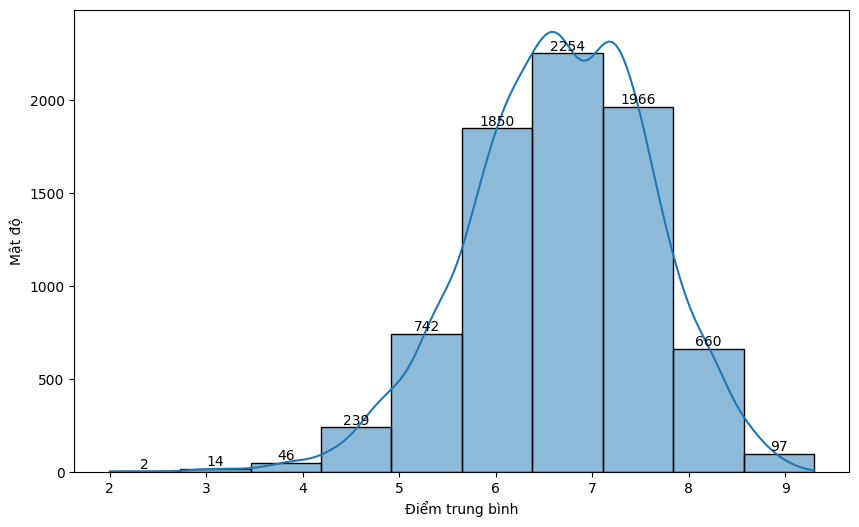
\includegraphics[width=0.90\textwidth]{images/Table_MAL_score.png}
        \caption{Phân phối điểm đánh giá trung bình }
        \label{fig:Table_MAL_score}
    \end{figure}

    \FloatBarrier
    
    Biểu đồ \ref{fig:Table_MAL_score} cho thấy phân phối điểm đánh giá trung bình có dạng chuẩn, đỉnh phân bố tập trung tại mức 6.5-7 điểm. Đường KDE gần như là hình chuông, đối xứng quanh trung tâm, cho thấy phần lớn phim đạt mức gần 7. Thực tế, người dùng thường cho điểm 6-7 cho phim mức trung bình thay vì 5, lý giải cho đỉnh phân phối lệch sang phải trên thang 0-10.

    \begin{figure}[htp]
        \centering
        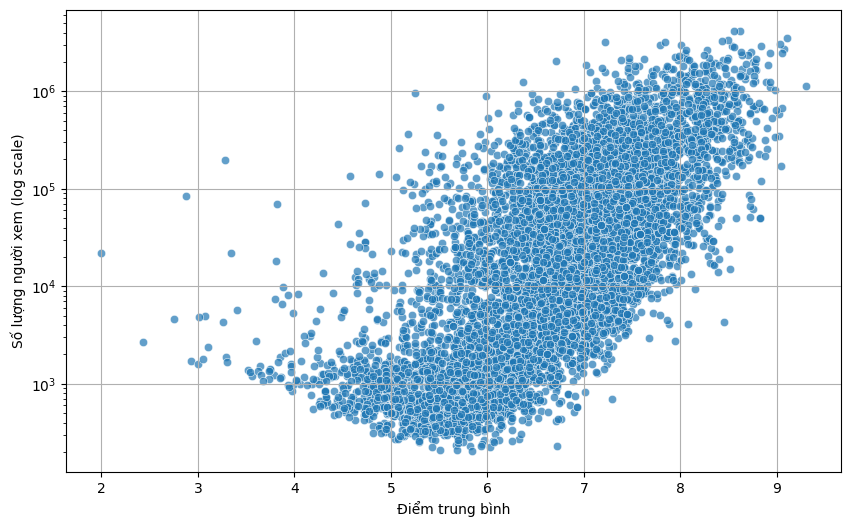
\includegraphics[width=0.90\textwidth]{images/Table_MAL_member_score.png}
        \caption{Số lượng người xem theo điểm}
        \label{fig:Table_MAL_member_score}
    \end{figure}

    \FloatBarrier

    Biểu đồ \ref{fig:Table_MAL_member_score} cho thấy số lượng người xem quan hệ chặt chẽ với đánh giá trung bình của phim. Đánh giá phim càng tốt thì càng nhiều người xem. 
    
    \begin{figure}[htp]
        \centering
        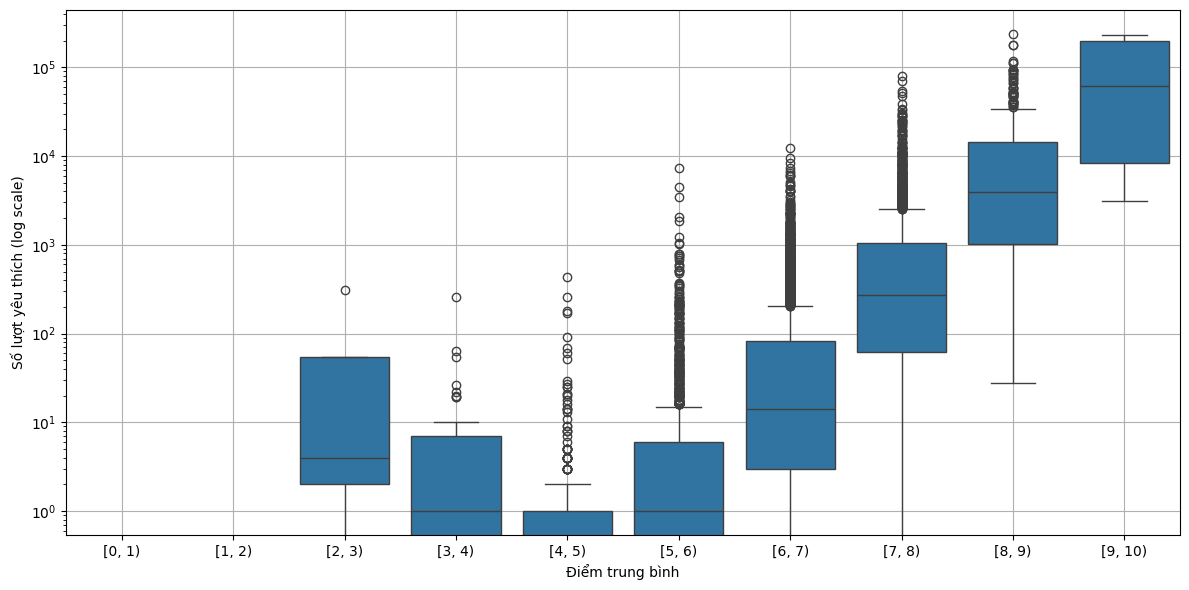
\includegraphics[width=0.90\textwidth]{images/Table_MAL_favorite_score.png}
        \caption{Số lượt yêu thích theo điểm}
        \label{fig:Table_MAL_favorite_score}
    \end{figure}

    \FloatBarrier

    Biểu đồ \ref{fig:Table_MAL_favorite_score} cho thấy số lượng liên hệ tích cực với điểm trung bình. Các boxplot lượt yêu thích ở mức điểm cao có trung vị cao hơn và khoảng tứ vị phân cũng cao hơn hẵn phần điểm thấp hơn. Tuy nhiên, có trường hợp ngoại lệ ở phần điểm thấp nhất lại có lượt yêu thích tương tự với phần điểm cho thấy phim ở mức trung bình 6-7. Điều này có thể giải thích bằng hiện tượng một số người sử dụng 'xem vì ghét' (hate-watching), hoặc phim 'dở quá đến mức hay' đối với một số người dùng, nên các phim được đánh giá rất thấp này có được một lượng yêu thích nhất định. Còn các phim chỉ dở bình thường, dù có đánh giá cao hơn nhưng không bắt được thị hiếu.

     \begin{figure}[htp]
        \centering
        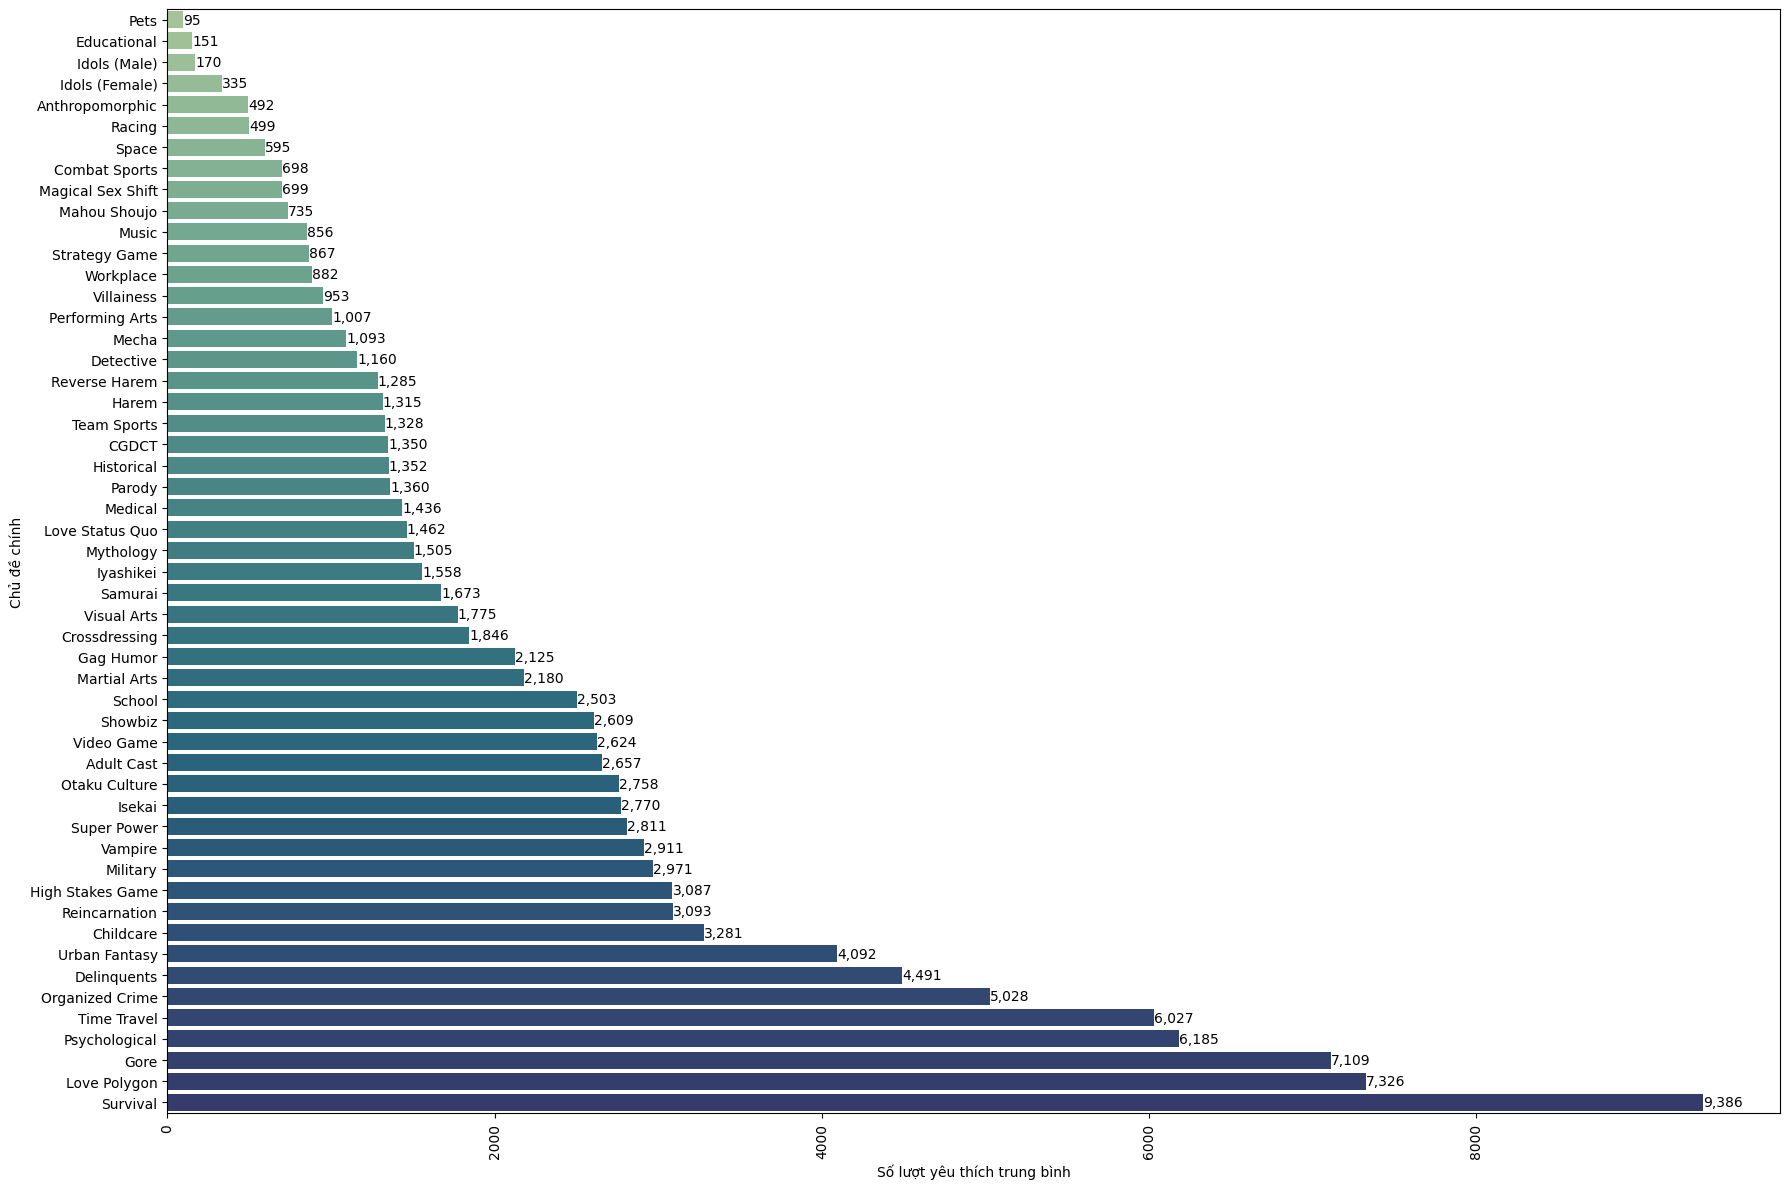
\includegraphics[width=0.90\textwidth]{images/Table_MAL_themes_fav.png}
        \caption{Số lượt yêu thích trung bình các chủ đề chính}
        \label{fig:Table_MAL_themes_fav}
    \end{figure}

    \FloatBarrier

    Biểu đồ \ref{fig:Table_MAL_themes_fav} thể hiện số lượt yêu thích trung bình giữa các chủ đề chính. Các chủ đề như 'Survival', 'Psychological' hay 'Time Travel' được yêu thích nhiều, cho thấy người xem chuộng nội dung căng thẳng, kịch tính. Trong khi đó, các chủ đề như 'Pets', 'Educational' hay 'Idols' ít được quan tâm, phản ánh xu hướng đa số không hứng thú với nội dung nhẹ nhàng.

    \begin{figure}[htp]
        \centering
        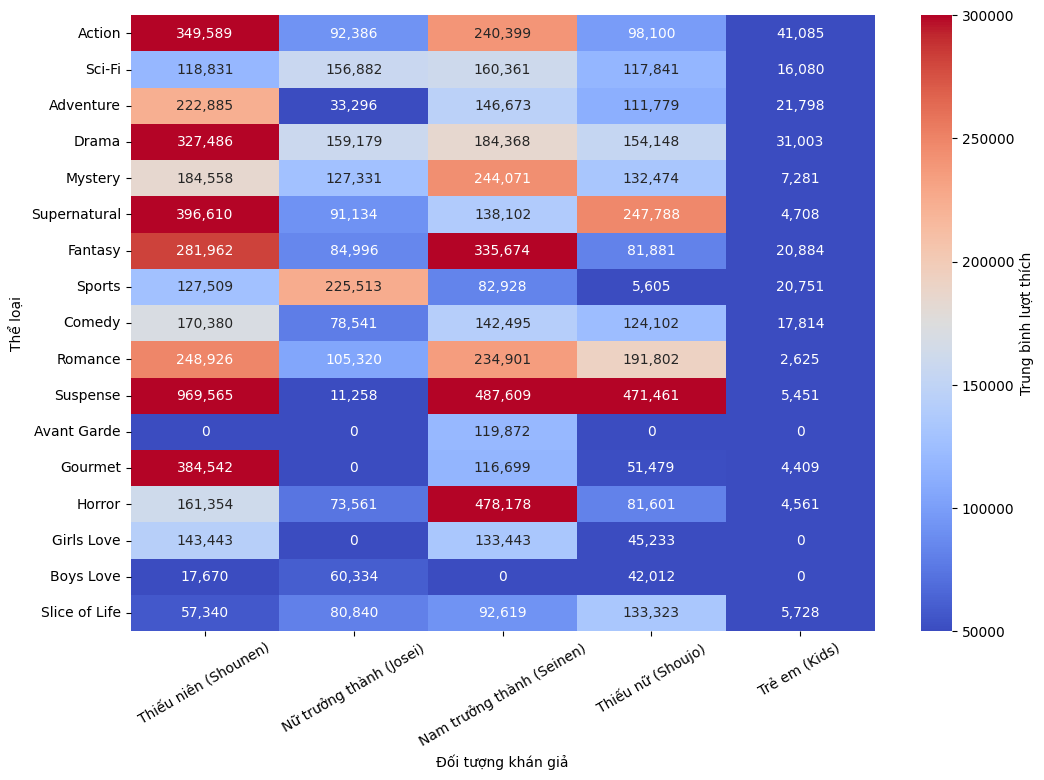
\includegraphics[width=0.90\textwidth]{images/Table_MAL_genre_demo_fav.png}
        \caption{Số lượt yêu thích trung bình các thể loại/đối tượng khán giả}
        \label{fig:Table_MAL_genre_demo_fav}
    \end{figure}

    \FloatBarrier

    Biểu đồ \ref{fig:Table_MAL_genre_demo_fav} thể hiện lượt yêu thích trung bình các thể loại phim theo từng nhóm đối tượng khán giả. Có thể thấy với từng nhóm khán giả yêu thích một số thể loại cụ thể, cho nên thể loại phim hợp với đối tượng khán giả hướng đến có ảnh hưởng lớn đến sự thành công của phim. Ở biểu đồ ta cũng thấy được, các phim hướng đối tượng trẻ em có lượt yêu thích rất thấp ở mọi thể loại.


\subsubsection{Mô hình hóa dữ liệu}
    \paragraph{Cấu hình cài đặt} 
    \leavevmode

    Các mô hình sử dụng:

    \begin{itemize}
        \item \textbf{Logistic Classification}: 

            \begin{lstlisting}[language=Python]
                LogisticRegressionCV(
                    max_iter=max_iter,
                    Cs=cs,
                )
            \end{lstlisting}

            khoảng hypertune tham số

            \begin{lstlisting}[language=Python]
                list_max_iter = [10, 20, 30, 40, 50, 100, 200, 300, 500]
                list_cs = [1,2,3,4,5,8,10]
            \end{lstlisting}.

        \item \textbf{Random Forest Classifier}:

            \begin{lstlisting}[language=Python]
                RandomForestClassifier(
                    max_depth=max_depth,
                    n_estimators=n_estimators,
                    min_samples_leaf=min_samples_leaf,
                )
            \end{lstlisting}

            khoảng hypertune tham số

            \begin{lstlisting}[language=Python]
                list_max_depth = [2, 3, 5, 10]
                list_n_estimators = [50, 100, 150, 200]
                list_min_samples_leaf = [3, 5, 10, 20]
            \end{lstlisting}.

        \item \textbf{XGBoost Classifier}:
            \begin{lstlisting}[language=Python]
                XGBClassifier(
                    max_depth=max_depth,
                    n_estimators=n_estimators,
                    reg_lambda=reg_lambda,
                    learning_rate=lr,
                    reg_alpha=alpha,
                )
            \end{lstlisting}

            khoảng hypertune tham số

            \begin{lstlisting}[language=Python]
                list_max_depth = [ 6, 7, 8, 9]
                list_lambda = [0.5, 1, 2]
                list_learning_rate = [1, 0.8, 0.5, 0.25]
                list_n_estimators = [50, 100, 150, 200]
                list_alpha = [0.5, 1, 2]
            \end{lstlisting}.
        
    \end{itemize}

    Thuật toán data transform sử dụng: Do dữ liệu có nhiều điểm ngoại lệ, nhóm chọn Robust Scaler để chuẩn hóa dữ liệu.

    Chia tập dữ liệu huấn luyện: Cross-validation 5 folds.
    

    \paragraph{Phân lớp đánh giá phim}
    \leavevmode

    Chuyển cột điểm trung bình giá về dạng nhãn. Dựa vào thống kê dữ liệu bảng \ref{tab:stat-mal}, phân phối điểm đánh giá hình \ref{fig:Table_MAL_score}, lượt yêu thích theo điểm \ref{fig:Table_MAL_favorite_score}, có thể chia nhãn điểm như sau
    \begin{itemize}
        \item Dưới 6: Bad - Tệ
        \item Từ 6-7: Ok - Ổn
        \item Từ 7-8: Good - Hay
        \item Trên 8: Great - Tuyệt vời
    \end{itemize}

    Phân phối nhãn điểm trên tập dữ liệu như hình \ref{fig:Table_MAL_score_label}

    \begin{figure}[htp]
        \centering
        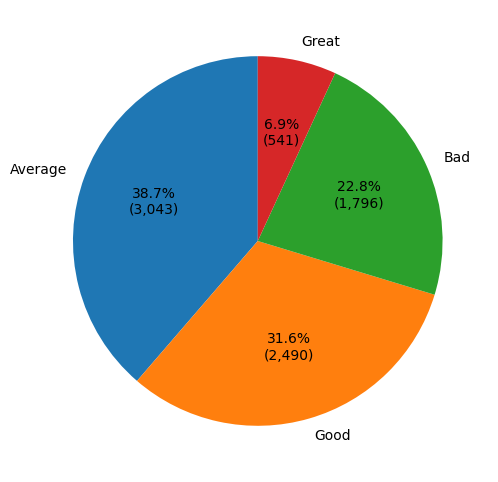
\includegraphics[width=0.80\textwidth]{images/Table_MAL_score_label.png}
        \caption{Phân phối nhãn điểm đánh giá}
        \label{fig:Table_MAL_score_label}
    \end{figure}

    \FloatBarrier

    Chọn các đặc trưng huấn luyện: 'genres' (one hot encoding), 'themes' (one hot encoding), 'studios' (category encoding)

    Kết quả:

    \begin{itemize}
        \item \textbf{Logistic Classification}: 
        
            Mô hình tốt nhất:
            \begin{itemize}
                \item max\_iter: 20
                \item cs: 5
            \end{itemize}

            \begin{table}[htbp]
            \centering
            \caption{Kết quả Logistic Classification - Phân lớp đánh giá}
            \label{tab:mal-score-LogCV}
            \begin{tabular}{lrrrrr}
                \hline
                & train\_acc & test\_acc & test\_recall & test\_precision & test\_f1 \\
                \hline
                mean & 0.576740 & 0.553721 & 0.452583 & 0.556177 & 0.475009 \\
                std & 0.004452 & 0.009356 & 0.014631 & 0.026914 & 0.020463 \\
                min & 0.571998 & 0.541833 & 0.434268 & 0.530762 & 0.451901 \\
                max & 0.582357 & 0.566301 & 0.473644 & 0.597646 & 0.505563 \\
                \hline
            \end{tabular}
            \end{table}
  
            
            \FloatBarrier
            
        \item \textbf{Random Forest Classifier}:

            Mô hình tốt nhất:
            \begin{itemize}
                \item max\_depth: 10
                \item n\_estimators: 150
                \item min\_samples\_leaf: 3
            \end{itemize}

            \begin{table}[htbp]
                \centering
                \caption{Kết quả Random Forest Classifier - Phân lớp đánh giá}
                \label{tab:mal-score-RF}
                \begin{tabular}{lrrrrr}
                    \hline
                     & train\_acc & test\_acc & test\_recall & test\_precision & test\_f1 \\
                    \hline
                    mean & 0.612567 & 0.574050 & 0.428677 & 0.648379 & 0.433171 \\
                    std & 0.003059 & 0.013495 & 0.016348 & 0.144203 & 0.019790 \\
                    min & 0.609367 & 0.553785 & 0.407844 & 0.481355 & 0.412235 \\
                    max & 0.616343 & 0.588235 & 0.451760 & 0.769657 & 0.463677 \\
                    \hline
                \end{tabular}
            \end{table}
            
            \FloatBarrier

        \item \textbf{XGBoost Classifier}:
        
            Mô hình tốt nhất:
            \begin{itemize}
                \item max\_depth: 7
                \item n\_estimators: 200
                \item reg\_lambda: 2
                \item reg\_alpha: 0.5
                \item learning\_rate: 0.5
            \end{itemize}

            \begin{table}[htbp]
                \centering
                \caption{Kết quả XGBoost Classifier - Phân lớp đánh giá}
                \label{tab:mal-score-XGBC}
                \begin{tabular}{lrrrrr}
                \hline
                 & train\_acc & test\_acc & test\_recall & test\_precision & test\_f1  \\
                \hline
                mean & 0.982310 & 0.707992 & 0.658002 & 0.696674 & 0.673979 \\
                std & 0.002217 & 0.013157 & 0.020672 & 0.016154 & 0.019047 \\
                min & 0.979566 & 0.691924 & 0.636567 & 0.675056 & 0.652368 \\
                max & 0.985052 & 0.722112 & 0.684336 & 0.713385 & 0.697402 \\
                \hline
                \end{tabular}
            \end{table}

            \FloatBarrier
    \end{itemize}

    So sánh các mô hình:

    \begin{table}[htbp]
        \centering
        \caption{So sánh kết quả các mô hình (và nghiên cứu liên quan) - Phân lớp đánh giá}
        \label{tab:mal-score-compare}
        \begin{tabular}{|p{2cm}|p{2cm}|p{2cm}|p{2cm}|p{2cm}|}
            \hline
             Model & Mean Test Accuracy & Mean F1 & Mean Recall & Mean Precision\\
            \hline
            Logistic Regression & 0.553721 & 0.475009 & 0.452583 & 0.556177 \\
            \hline
            Random Forest & 0.574050 & 0.433171 & 0.428677 & 0.648379 \\
            \hline
            XGBoost & \textbf{0.707992} & \textbf{0.673979} & \textbf{0.658002} & 0.696674 \\
            \hline
             BBTC, LogReg* \cite{armenta2023anime} & 0.60 & 0.55 & 0.64  &  0.48  \\
            \hline
            BoW, NB** \cite{armenta2023anime} & 0.5 & 0.66 & 0.5  &  \textbf{1}  \\
            \hline
        \end{tabular}
    \end{table}

    \FloatBarrier

    \textit{(*): Bag of Words, Bigrams, Trigrams, Character Trigrams + Logistic Regression}

    \textit{(**): Bag of Words + Naive Bayes}

    Trong bài toán phân lớp đánh giá, Logistic Regression và Random Forest cho kết quả thấp hơn đáng kể, độ chính xác chỉ tầm 0.55, 0.57. Dặc biệt F1 và Recall đều dưới mức 0.5 ở cả 2 mô hình. Cho thấy đây là bài toán phân lớp phức tạp khiến hai mô hình đơn giản hơn này cho kết quả không tốt. Mô hình XGBoost thể hiện rõ rệt sự vượt trội so với các mô hình khác, đạt độ chính xác $\approx$ 0.708, f1 $\approx$ 0.674, recall 0.658 và precision $\approx$ 0.697. Đây là mô hình duy nhất đạt đồng thời kết quả cao ở cả bốn chỉ số, cho thấy một phần hiệu quả trong việc phân lớp. Tuy có độ chính xác trên tập test gần 0.708, bảng \ref{tab:mal-score-XGBC} cho thấy độ chính xác huấn luyện mô hình đến 0.98, cho thấy dữ liệu nhiễu cao và mô hình đang bị overfit. Mô hình XGBoost thu được cũng có các kết quả đa phần cao hơn hai mô hình từ nghiên cứu của Armenta và cộng sự \cite{armenta2023anime}.

    \FloatBarrier

    \paragraph{Phân lớp đánh giá độ phổ biến}
    \leavevmode

    Để xác định độ phổ biến của phim, ta có thể dựa vào cột 'members', số lượng người xem. Chuyển cột 'members' về nhãn, đầu tiên áp dụng hàm logarithm để giảm độ lớn hiện có của dữ liệu, sau đó ta có thể sử dụng các phân vị để tạo 4 nhãn có phân phối bằng này.:

    \begin{lstlisting}[language=Python]
    df_processed['log_members'] =  p.log1p(df_processed['members'])
    
    df_processed['members_label_as_int'] = pd.qcut(
        df_processed['log_members'],
        q=4,
        labels=[0, 1, 2, 3]
    ).astype(int)
    \end{lstlisting}

    Kết quả:

    \begin{itemize}
        \item \textbf{Logistic Classification}: 
        
            Mô hình tốt nhất:
            \begin{itemize}
                \item max\_iter: 100
                \item cs: 5
            \end{itemize}

            \begin{table}[htbp]
            \centering
            \caption{Kết quả Logistic Classification - Phân lớp độ phổ biến}
            \label{tab:mal-member-LogCV}
            \begin{tabular}{lrrrrr}
                \hline
                & train\_acc & test\_acc & test\_recall & test\_precision & test\_f1 \\
                \hline
                mean & 0.575792 & 0.546939 & 0.537928 & 0.551536 & 0.541903 \\
                std & 0.004049 & 0.008926 & 0.009028 & 0.011581 & 0.008809 \\
                min & 0.570752 & 0.535394 & 0.528976 & 0.534441 & 0.533827 \\
                max & 0.581216 & 0.558765 & 0.547981 & 0.567014 & 0.554310 \\
                \hline
            \end{tabular}
            \end{table}
  
            
            \FloatBarrier
            
        \item \textbf{Random Forest Classifier}:

            Mô hình tốt nhất:
            \begin{itemize}
                \item max\_depth: 10
                \item n\_estimators: 200
                \item min\_samples\_leaf: 3
            \end{itemize}

            \begin{table}[htbp]
                \centering
                \caption{Kết quả Random Forest Classifier - Phân lớp phổ biến}
                \label{tab:mal-member-RF}
                \begin{tabular}{lrrrrr}
                    \hline
                     & train\_acc & test\_acc & test\_recall & test\_precision & test\_f1 \\
                    \hline
                        mean & 0.615706 & 0.565880 & 0.545500 & 0.595757 & 0.558836 \\
                        std & 0.002279 & 0.011968 & 0.015212 & 0.009591 & 0.013481 \\
                        min & 0.612759 & 0.546813 & 0.524157 & 0.582396 & 0.541538 \\
                        max & 0.618087 & 0.579262 & 0.565344 & 0.608816 & 0.575794 \\
                    \hline
                \end{tabular}
            \end{table}
            
            \FloatBarrier

        \item \textbf{XGBoost Classifier}:
        
            Mô hình tốt nhất:
            \begin{itemize}
                \item max\_depth: 8
                \item n\_estimators: 50
                \item reg\_lambda: 2
                \item reg\_alpha: 0.5
                \item learning\_rate: 0.5
            \end{itemize}

            \begin{table}[htbp]
                \centering
                \caption{Kết quả XGBoost Classifier - Phân lớp độ phổ biến}
                \label{tab:mal-member-XGBC}
                \begin{tabular}{lrrrrr}
                \hline
                 & train\_acc & test\_acc & test\_recall & test\_precision & test\_f1  \\
                \hline
                mean & 0.886237 & 0.613711 & 0.616620 & 0.626318 & 0.620354 \\
                std & 0.002355 & 0.009508 & 0.005633 & 0.014513 & 0.008927 \\
                min & 0.882382 & 0.599202 & 0.609210 & 0.604851 & 0.606661 \\
                max & 0.888391 & 0.625498 & 0.622128 & 0.642860 & 0.629061 \\
                \hline
                \end{tabular}
            \end{table}

            \FloatBarrier
    \end{itemize}

    So sánh các mô hình:

    \begin{table}[htbp]
        \centering
        \caption{So sánh kết quả các mô hình - Phân lớp độ phổ biến}
        \label{tab:mal-member-compare}
        \begin{tabular}{|p{4cm}|p{2cm}|p{2cm}|p{2cm}|p{2cm}|}
            \hline
             Model & Mean Test Accuracy & Mean F1 & Mean Recall & Mean Precision\\
            \hline
            Logistic Regression & 0.546939 & 0.541903 & 0.537928 & 0.551536 \\
            \hline
            Random Forest & 0.565880 & 0.558836 & 0.545500 & 0.595757 \\
            \hline
            XGBoost & \textbf{0.613711} & \textbf{0.620354} & \textbf{0.616620} & \textbf{0.626318} \\
            \hline
        \end{tabular}
    \end{table}

    \FloatBarrier

    Mô hình Logistic Regression và Random Forest tiếp tục cho kết quả thấp hơn đáng kể, độ chính xác chỉ tầm 0.54, 0.56. Tuy nhiên không có chỉ số nào có kết quả dưới 0.5 như bài phân lớp đánh giá trước. Mô hình XGBoost tiếp tục thể hiện rõ rệt sự vượt trội so với các mô hình khác, đạt độ chính xác $\approx$ 0.61, f1 0.62, recall $\approx$ 0.62 và precision $\approx$ 0.62. 

    \paragraph{Phân lớp đánh giá độ yêu thích}
    \leavevmode

    Để xác định độ yêu thích của phim, ta có thể dựa vào cột 'favorites', số lượng người xem. Chuyển cột 'favorites' về nhãn, đầu tiên áp dụng hàm logarithm để giảm độ lớn hiện có của dữ liệu, sau đó ta có thể sử dụng các phân vị để tạo 4 nhãn có phân phối bằng này.:

    \begin{lstlisting}[language=Python]
    df_processed['favorites'] =  p.log1p(df_processed['favorites'])
    
    df_processed['favorites_label_as_int'] = pd.qcut(
        df_processed['log_favorites'],
        q=4,
        labels=[0, 1, 2, 3]
    ).astype(int)
    \end{lstlisting}

    Kết quả:

    \begin{itemize}
        \item \textbf{Logistic Classification}: 
        
            Mô hình tốt nhất:
            \begin{itemize}
                \item max\_iter: 10
                \item cs: 4
            \end{itemize}

            \begin{table}[htbp]
            \centering
            \caption{Kết quả Logistic Classification - Phân lớp độ yêu thích}
            \label{tab:mal-fav-LogCV}
            \begin{tabular}{lrrrrr}
                \hline
                & train\_acc & test\_acc & test\_recall & test\_precision & test\_f1 \\
                \hline
                mean & 0.541758 & 0.516247 & 0.502026 & 0.506926 & 0.502540 \\
                std & 0.004543 & 0.015478 & 0.014786 & 0.014137 & 0.014253 \\
                min & 0.536506 & 0.491036 & 0.481737 & 0.484314 & 0.482091 \\
                max & 0.546723 & 0.529880 & 0.515479 & 0.519512 & 0.515302 \\
                \hline
            \end{tabular}
            \end{table}
  
            
            \FloatBarrier
            
        \item \textbf{Random Forest Classifier}:

            Mô hình tốt nhất:
            \begin{itemize}
                \item max\_depth: 10
                \item n\_estimators: 50
                \item min\_samples\_leaf: 5
            \end{itemize}

            \begin{table}[htbp]
                \centering
                \caption{Kết quả Random Forest Classifier - Phân lớp yêu thích}
                \label{tab:mal-fav-RF}
                \begin{tabular}{lrrrrr}
                    \hline
                     & train\_acc & test\_acc & test\_recall & test\_precision & test\_f1 \\
                    \hline
                    mean & 0.541061 & 0.503890 & 0.464455 & 0.534843 & 0.471668 \\
                    std & 0.008845 & 0.023235 & 0.021512 & 0.021478 & 0.022017 \\
                    min & 0.526408 & 0.468127 & 0.434337 & 0.497847 & 0.441626 \\
                    max & 0.549327 & 0.524900 & 0.485608 & 0.549807 & 0.493303 \\
                    \hline
                \end{tabular}
            \end{table}
            
            \FloatBarrier

        \item \textbf{XGBoost Classifier}:
        
            Mô hình tốt nhất:
            \begin{itemize}
                \item max\_depth: 7
                \item n\_estimators: 200
                \item reg\_lambda: 2
                \item reg\_alpha: 0.5
                \item learning\_rate: 0.25
            \end{itemize}

            \begin{table}[htbp]
                \centering
                \caption{Kết quả XGBoost Classifier - Phân lớp độ yêu thích}
                \label{tab:mal-fav-XGBC}
                \begin{tabular}{lrrrrr}
                \hline
                 & train\_acc & test\_acc & test\_recall & test\_precision & test\_f1  \\
                \hline
                mean & 0.898395 & 0.561888 & 0.560000 & 0.558003 & 0.558385 \\
                std & 0.004875 & 0.007222 & 0.012267 & 0.008956 & 0.010239 \\
                min & 0.894121 & 0.554337 & 0.544279 & 0.546286 & 0.544556 \\
                max & 0.905331 & 0.569721 & 0.577044 & 0.567922 & 0.570822 \\
                \hline
                \end{tabular}
            \end{table}

            \FloatBarrier
    \end{itemize}

    So sách các mô hình:

    \begin{table}[htbp]
        \centering
        \caption{So sánh kết quả các mô hình - Phân lớp độ yêu thích}
        \label{tab:mal-fav-compare}
        \begin{tabular}{|p{2cm}|p{2cm}|p{2cm}|p{2cm}|p{2cm}|}
            \hline
             Model & Mean Test Accuracy & Mean F1 & Mean Recall & Mean Precision\\
            \hline
            Logistic Regression & 0.516247 & 0.502540 & 0.502026 & 0.506926 \\
            \hline
            Random Forest & 0.503890 & 0.471668 & 0.464455 & 0.534843 \\
            \hline
            XGBoost & \textbf{0.561888} & \textbf{0.558385} & \textbf{0.560000} & \textbf{0.558003} \\
            \hline
        \end{tabular}
    \end{table}

    \FloatBarrier

    Các mô hình đều cho kết quả khá thấp. Mô hình Logistic Regression và Random Forest thấp hơn đáng kể, độ chính xác chỉ tầm 0.51, 0.5. Mô hình Random Forest có F1 và Recal dưới 0.5. Mô hình XGBoost cho kết quả tốt hơn chút ít so với các mô hình khác, đạt độ chính xác 0.56, f1 0.55, recall 0.56 và precision 0.558. 

\subsubsection{Kết luận}
    Trong nghiên cứu này, nhóm đã phân tích và mô hình hóa phân lớp đánh giá, độ phổ biến và độ yêu thích của các bộ phim bộ dữ liệu MAL dataset. Kết quả cho thấy XGBoost luôn cho kết quả cao nhất, đạt độ chính xác cao nhất ở cả ba bài toán, đặc biệt là phân loại đánh giá với accuracy 0.708 và F1 0.674. So với nghiên cứu liên quan, mô hình thu được là cải tiến. Tuy nhiên, hiện tượng overfitting và kết quả thấp ở bài toán độ yêu thích cho thấy cần cải thiện thêm về tiền xử lý dữ liệu và mô hình hóa, cho thấy các đặc trưng hành vi được lựa chọn có mối quan hệ rõ ràng và có khả năng phân biệt tốt giữa các lớp tính cách.

